\lecture{Simulazione di un Digital Twin}{17~-~01~-~2026}
%
%
\section{Modelli e sistemi}
Per costruire un DT è necessario partire dalle basi della modellazione.
%
\paragraph{Definizione di modello} Un modello è una rappresentazione di un sistema reale che ne riproduce le proprietà rilevanti. Non è la realtà stessa, ma un'astrazione utile.
%
\subsection{Strategie di Modellazione}
Distinguiamo tre approcci principali basati sul livello di conoscenza del sistema e sul controllo desiderato sul modello: i primi due sono il White Box Modeling ed il Black Box Modeling, mentre il terzo è l'Hybrid Analysis and Modeling, una possibile futura direzione che combina i primi due sistemi insieme.
%
\subsubsection{White Box Modeling}
Si basa sulla conoscenza fisica completa del sistema. Usa leggi fisiche modellate con equazioni matematiche per riprodurre fenomeni (es. analisi cinematica, termica, fluidodinamica \dots).

Vedi tabella \ref{tab:wbm} per i pro e i contro e figura \ref{fig:07-whitebox}.
%
\begin{table}
    \centering
    \begin{tabularx}{0.8\linewidth}{>{\parskip1ex}X@{\kern4\tabcolsep}>{\parskip1ex}X}
        \toprule
        \hfil\bfseries Pros
         &
        \hfil\bfseries Cons
        \\\cmidrule(r{3\tabcolsep}){1-1}\cmidrule(l{-\tabcolsep}){2-2}

        %% PROS, ...\par
        Altissima interpretabilità (si capisce il perché di un comportamento) \par

         &

        %% CONS, ...\par
        Richiede conoscenza avanzata del sistema \par
        È molto oneroso computazionalmente e lento da costruire\par
        È comunque un'approssimazione: se le ipotesi fisiche sono errate, il modello è parziale\par
        \\\bottomrule
    \end{tabularx}
    \caption{White Box Modeling Pros and Cons}\label{tab:wbm}
\end{table}

\begin{example}[White Box Modeling]
    Modellazione geometrica/CAD (AutoCAD, SolidWorks) per definire dimensioni, collisioni e cinematica.
\end{example}

\begin{figure}
    \centering
    \begin{minipage}{0.45\textwidth}
        \centering
        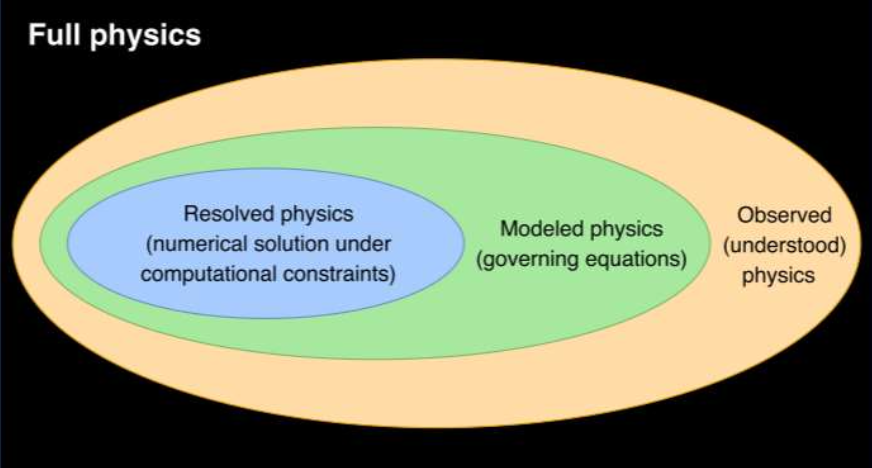
\includegraphics[width=\linewidth]{assets/Screenshot 2026-01-17 at 20.07.08.png}
        \caption{White Box}
        \label{fig:07-whitebox}
    \end{minipage}
    \begin{minipage}{0.45\textwidth}
        \centering
        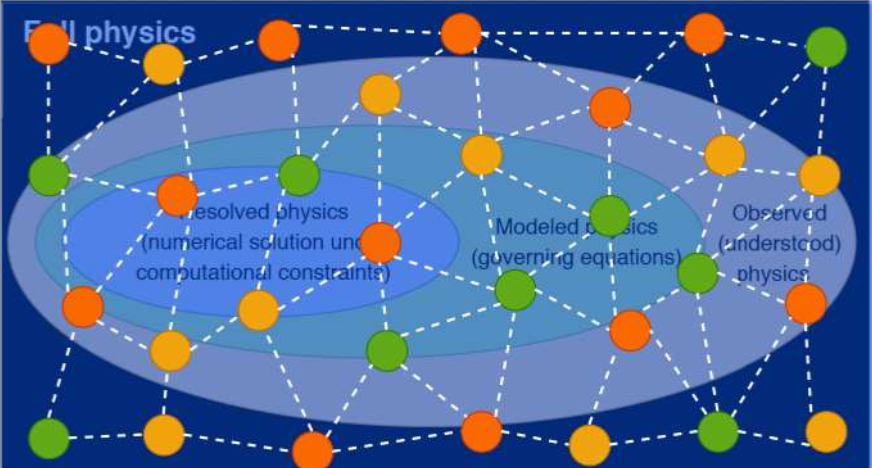
\includegraphics[width=\linewidth]{assets/Screenshot 2026-01-17 at 20.09.01.png}
        \caption{Black Box (data-driven)}
        \label{fig:07-blackbox}
    \end{minipage}
\end{figure}

\subsubsection{Black Box Modeling}
Si basa esclusivamente sui dati disponibili, senza conoscenza a priori della fisica sottostante.
Rappresenta il comportamento input/output per minimizzare l'errore su una metrica specifica. Utile quando la fisica è troppo complessa o ignota.
%
\begin{table}
    \centering
    \begin{tabularx}{0.8\linewidth}{>{\parskip1ex}X@{\kern4\tabcolsep}>{\parskip1ex}X}
        \toprule
        \hfil\bfseries Pros
         &
        \hfil\bfseries Cons
        \\
        \cmidrule(r{3\tabcolsep}){1-1}\cmidrule(l{-\tabcolsep}){2-2}

        %% PROS, ...\par
        Molto veloce da costruire e da eseguire\par
        Non richiede conoscenza dettagliata del fenomeno\par

         &

        %% CONS, ...\par
        Non è interpretabile (``scatola nera'', difficile capire il perché di una decisione)\par
        dipende fortemente dalla qualità e quantità dei dati.\par

        \\
        \bottomrule
    \end{tabularx}
    \caption{Black Box Modeling Pros and Cons}\label{tab:bbm}
\end{table}
%
\paragraph{Approcci} Due approcci principali al Black Box Modeling: modelli statistici (Catene di Markov) o Machine Learning (Reti Neurali).

Vedi tabella \ref{tab:bbm} per i pro e contro e figura \ref{fig:07-blackbox}.
%
\subsubsection{Hybrid Analysis and Modeling}
La direzione futura che combina i due approcci per superare i limiti di entrambi. L'obiettivo è unire l'interpretabilità e la robustezza dei modelli fisici con l'accuratezza ed efficienza dei modelli guidati dai dati (data-driven).
%
\paragraph{Tecniche} Uso di modelli ``surrogati'', ML informato dalla fisica, o modelli a ordine ridotto.

Vedi figura \ref{fig:07-ham}.
\begin{figure}
    \centering
    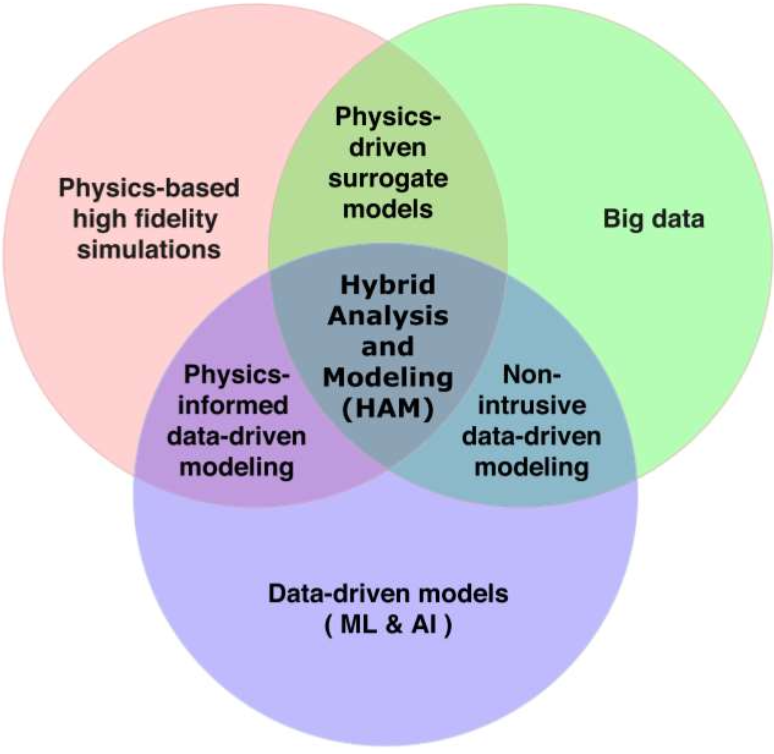
\includegraphics[width=0.5\linewidth]{assets/Screenshot 2026-01-17 at 20.06.46.png}
    \caption{}\label{fig:07-ham}
\end{figure}

%
\section{Livelli di Simulazione}
Il DT può essere modellato a diversi livelli di granularità:
\begin{enumerate}
    \item Unit Level: Singolo equipaggiamento o isola di produzione (dettaglio elevato, anche meccanico);
    \item System Level: Intera linea di produzione o impianto (focus su flussi e interconnessioni);
    \item System of Systems Level: Integrazione a livello di impresa (Supply Chain, intero ciclo di vita).
\end{enumerate}
%
\subsection{Industry-level Tools}
%
\paragraph{Siemens Plant Simulation} Per simulazione a livello di sistema (flussi, logistica, colli di bottiglia). Vedi figura \ref{fig:07-siemens}.
%
\paragraph{Ansys Twin Builder} Per simulazione multi-fisica ad alta fedeltà. Vedi figura \ref{fig:07-ansys}.


\begin{figure}
    \centering
    \begin{subfigure}{0.48\linewidth}
        \centering
        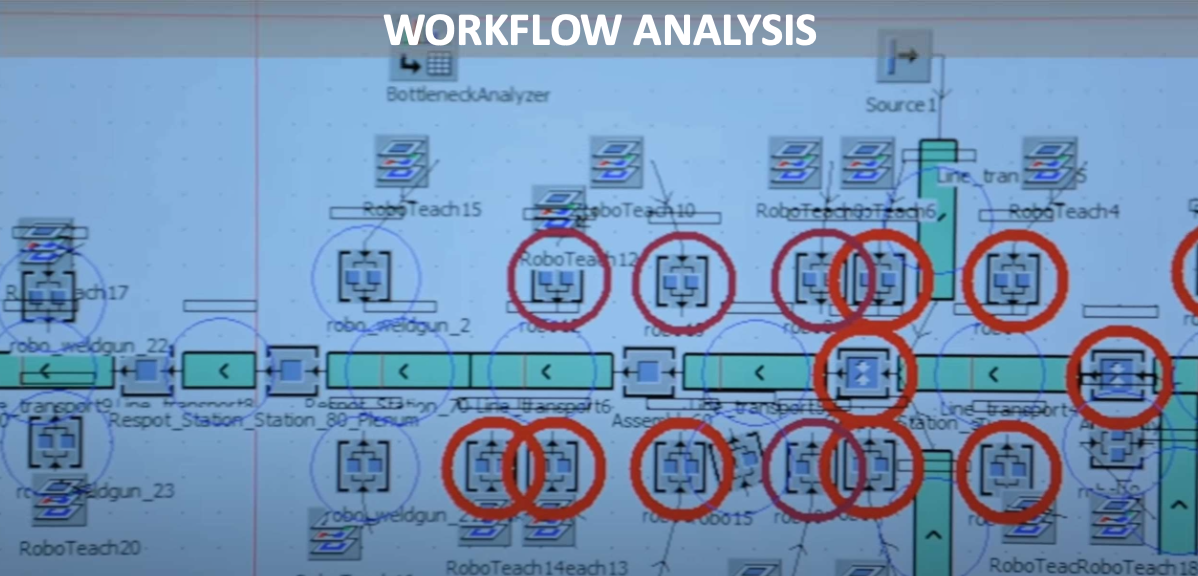
\includegraphics[width=\linewidth]{assets/Screenshot 2026-01-17 at 20.16.33.png}
        \caption{Siemens Plant Simulation}\label{fig:07-siemens}
    \end{subfigure}
    \begin{subfigure}{0.45\linewidth}
        \centering
        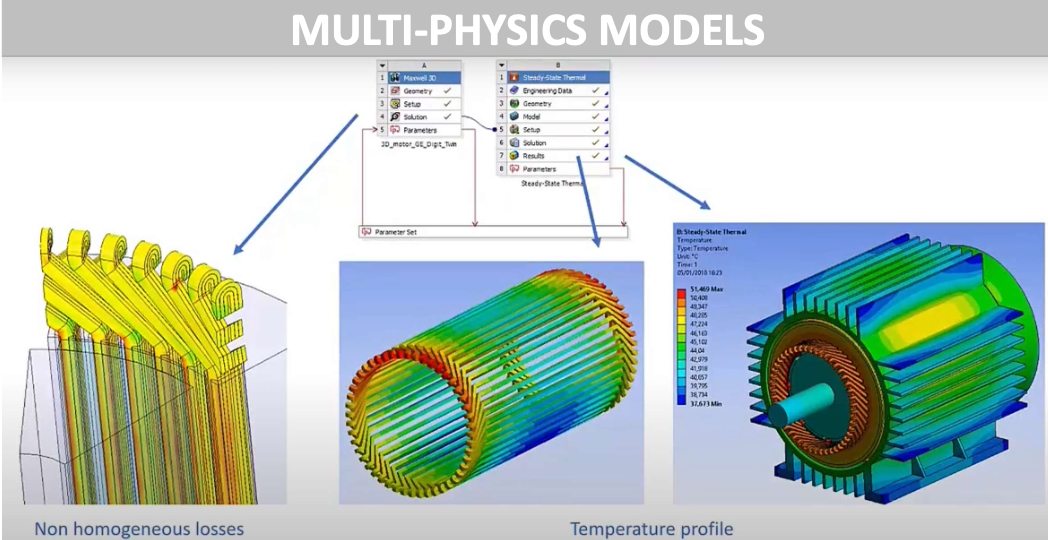
\includegraphics[width=\linewidth]{assets/Screenshot 2026-01-17 at 20.15.53.png}
        \caption{Ansys Twin Builder}\label{fig:07-ansys}
    \end{subfigure}
    \caption{Industry-level tools}\label{fig:07-tools}
\end{figure}